% !TeX root = SketchFace.tex

% 
\begin{figure}
	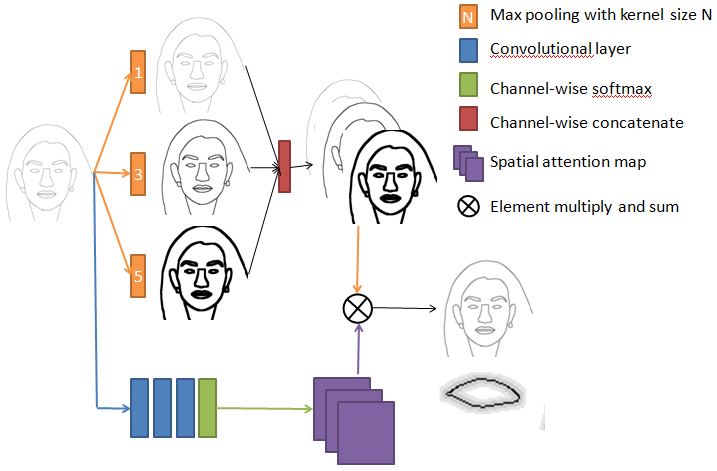
\includegraphics[width=\columnwidth]{figs/sap.png}
	\caption{Sap}
	\label{fig:sap}
\end{figure}
%

\subsubsection{Spatial Attention Pooling}
\label{subsec:algorithm_sap}
\td{(Check if the idea about the relax is well-described)}
\td{(Spatial-specific?Position-specific?Spatially variant?)}
When a input hand-drawn sketch is not well-drawn, line distortions of the sketch damages the quality of the generated face image. Tt is a trade-off between the realism of the output face image and the alignment between the input sketch and the output face image.
%
In order to alleviate the edge alignment between the input sketch and the output face image, we desire to relax thin strokes to ambiguity bands with various width or uncertainty.
One of the straightforward ways is to smooth the lines of sketches using image smoothing algorithm. 
\td{Another is to dilate the sketch lines so that the widths of lines are of multiple pixels~\cite{DeepSurgery}.}
%
However, the capacity of either the two hand-crafted ways above is limited, because the uniform smoothness \td{and the dilate radius} for all positions of the whole sketch violate the unevenness of hand-drawn sketches on depicting different facial parts. 
%
We argue that the balance between the realism of the output face image and the alignment between the input sketch and the output face image differs from one position to another across the face image. Therefore, the relax degree should be spatial-specific. 

Based on the discussion above, we propose a new module, called spatial attention pooling (SAP), to adaptively relax the widths of strokes in the input sketch in a spatial-specific way. 
\cxj{I would not use 'dilate' since this simple word does not reveal the underlying discovery.}
%Let $\mathbf{r}=\{r_i | i=1,2,...,N_r\}$ be a set of relax radius. 
Given an input sketch $S\in \real^{H\times W}$, we first pass it through $N_r$ pooling branches with different kernel sizes of $\{r_i, i=1,\ldots, N_r\}$ to get $\{P_{i}| i=1,\ldots,N_r\}$. 
In order to get a relaxed sketch $\tilde{S}$ with spatial-specific stroke widths, we compute
%	
\begin{equation}
\tilde{S}=\sum_{i=1}^{N_r} A_i * P_{r_i}(s),
\end{equation}
%
where $*$ is element-wise multiplication and $A_i$ is the $ith$ channel of the spatial attention map $A\in \real^{N_r\times H\times W}$.
The spatial attention map $A$ controls the relax degrees of all positions of the input sketch.
Since a line with a large distortion is supposed to be assigned with a large relax degree, $A$ is supposed to adaptively pay more attention (a large value) to a $P_i$ with a large kernel size in the areas with large line distortions.
%

%
A straightforward way to get $A$ is passing the input sketch through a few convolutional layers and these convolutional layers are trained to detect the areas with line distortions. However, we found the a few convolutional layers are insufficient to learn to detect line distortions directly. Therefore, we introduce a two-class classifier to ease the detection. Specifically, we pre-train a fully-convolutional two-class classifier $C$ with three convolutional layers to distinguish sketches from deformed sketches. Then we utilize this pre-trained classifier to extract features of the input sketch $S$ to get ${C_i(S), i=1,2,3}$, where $C_i(·)$ denotes the $ith$ feature maps extracted by $C$. These feature maps from classifier emphasize the differences between sketches and deform sketches. We resize and concatenate these feature maps, and pass them through three convolutional layers to get the spatial attention map:
%	
\begin{equation}
A=Softmax(Conv([C_1, Up_2(C_2), Up_4(C_3)])), 
\end{equation}
%
where $Up_2$ and $Up_4$ indicates $2\times$ and $4\times$ upsampling, Conv(·) indicates three cascaded convoutional layers, and $Softmax(·)$ is a softmax layer computed over channels to ensuring that for each position of $A$, the sum of weights of all channels equals to $1$.



We show this idea in Fig.~\ref{fig:sap}.




